\chapter{Change-point detection for concentration data}\label{chp:4}

\minitoc

\clearpage

In this Chapter, we build a change-point detection algorithm specially adapted for concentration data. We will use that algorithm to detect homogeneous temporal periods of times on which spatial statistical inferences will be possible. Several elements presented in Chapter \ref{chp:3} are used to build this method:  
\begin{itemize}
\item We use a parametric change-point detection, more precisely a maximum likelihood based method. The cost function $W$ is defined as the negative log likelihood of a distribution $Q$. The choice of $Q$ is motivated by the observation of the data, see Chapter \ref{chp:5} for an illustration on pesticide concentration data modeling.  
\item We use the PELT search method to obtain optimal solution to the change-point detection problem. Several penalty values $\beta$ are explored with the CROPS algorithm. The elbow method is applied when it is necessary to estimate an optimal number of change-points.   
\end{itemize}
We first describe the model integrating the censorship information in Section \ref{chp:4:1}. However, we don't known how much the censorship can affect a parametric change-point model. We provde a study of censoring effects in Section \ref{chp:4:2}. Futhermore, we need to devise a estimation procedure that is adapted to the observations of pesticide concentrations. The question sums up to detecting breaks in all dimensions of the parameters of $Q$ or not. We devise our estimation scheme in Section \ref{chp:4:3}. Finally we test our method with a change-point method adapted for censored data in Section \ref{chp:4:4}.  


\section{Generic model for censored data}\label{chp:4:1}

We present here the underlying parametric model we are using. We condider $\bm c = c_1,\dots,c_n$ that are realizations of independant random variables $C_1,\dots,C_n$. The variables $C_i$ are recorded sequentially, and the recording times are not necessarily equidistant. Thus, the indices in $Y_i$ are only indicators of the order of occurrence in the sample and not of the observation times. We suppose that there exist $K^*$ changes in the distribution of $\bm c$ happening at index $0=\tau_0^*<\tau^*_1 <... < \tau^*_k <... < \tau^*_{K^*}<\tau^*_{K^*+1}=n$. Moreover, on the k-th segment, $C_{\tau^*_{k-1}+1:\tau^*_{k}}$ follows a distribution $Q$ with parameters defined by the vector $\theta^*_k\in\Theta$ with $\Theta\subset\mathbb{R}^p$. We denote $\bm{\theta^*} = (\theta^*_k)_{k=0}^{K^*}$. More formally, we have that:  
$$c_t \sim f(.;\theta^*_k)\mathbbm{1}_{\tau^*_{k}+1\leq t \leq \tau^*_{k+1}},$$
with $f$ being the density function of distribution $Q$.  


The observations are subject to censorship. We focus on left-censorship because it is adapted for modeling concentration data but similar models can be created for right censorship or a mix of both. To each $c_i$ is associated a known censoring threshold $a_i$. The resulting censored observations are defined by:  
\begin{equation}\label{chp:4:defy}
Y_i = \sup(C_i,a_i)
\end{equation}
Since the $C_i$ are independant and the $a_i$ are known deterministic values, the $Y_i$ are independant as well. Noting $F$ the cumulative distribution function (cdf) of $Q$, we can write the cost function associted to segment $y_{u:v}$ as:  
\begin{equation}\label{chp:4:costfunc}
W(y_{u:v}) = -\sup_{\theta \in \Theta}\{\sum_{i=u}^v\log(F(y_i,\theta))\mathbbm{1}_{y_i=a_i}+\sum_{i=u}^v\log(f(y_i,\theta))\mathbbm{1}_{y_i>a_i}\}
\end{equation}
Note that if one needs to integrate right censorship into the likelihood, one should simply replace the $\sup$ in the definition \ref{chp:4:defy} by the $\inf$ of both quantities and cdf function $F$ by the survival function $S(t)=1-F(t)$. 
For a segmentation $\TT = \{\tau_1,...,\tau_K\}$, the penalised cost is given by: 
\begin{equation}\label{chp:4:pencost}
\CC(\bm y,\TT)=\sum_{i=0}^{K}  W(y_{\tau_i+1:\tau_{i+1}}) + Kp\beta,
\end{equation}
where $p$ is the dimension of the parameters vector in the distribution $Q$. Gathering \ref{chp:4:costfunc} and \ref{chp:4:pencost}, this resulting estimator can be expressed as:  
\begin{equation}\label{chp:4:estim}
(\widehat{\TT},\widehat{\bm \theta}) = \arg\min_{\TT,\bm \theta} \left(- \sum_{i=0}^{\lvert \TT \rvert}  \left\{\sum_{j=\tau_i+1}^{\tau_{i+1}}\log(F(y_j,\theta))\mathbbm{1}_{y_j=a_j}+\sum_{j=\tau_i+1}^{\tau_{i+1}}\log(f(y_j,\theta))\mathbbm{1}_{y_j>a_j}\right\}+\beta Kp\right)
\end{equation}

Under this configuration, we know that the estimators computed \ref{chp:4:estim} have satisfying convergence properties \citep{Lavielle1997}. A small proof is provided in Appendix \ref{app:chap4}.

\section{Censorship effects}\label{chp:4:2}

We are interested in the effects of censorship on two main aspects: 
\begin{itemize}
\item The estimation of the parameters $\bm \theta$ of $Q$ on a fixed segment. 
\item The implication it can have on the search method PELT and how to adapt it if this is the case. 
\end{itemize} 
Illustrating examples are provided in this section with $Q$ set as the exponential distribution.

\subsection{On the parameter estimation for one segment}

In general, an explicit formula for the maximum likelihood estimator (MLE) is not available in presence of censored data, leading to the use of numerical methods for its computation. The Newton-Raphson method was used on each segment to compute the MLE estimate of $\theta$. The cost functions need to be twice differentiable in $\theta$. We search for the zeros of the first derivate of the cost function in order to find a global minimum. 

Checking that the second derivative is strictly positive in presence of censored data, thus guaranteeing the unicity of the maximum likelihood estimate, can prove to be a difficult task as it is not always the case for all distribution $Q$. We provide an example of such a case in Appendix where we prove the existence of a global minimum without having the global convexity of the first derivate. This implies that a careful initialization of the Newton-Raphson method to obtain convergence. Appendix also provide experiments on the initialization of the Newton-Raphson method. 

FInally, the case where all data in the segment $y_{u:v}$ are censored is problematic. Looking at the analytical likelihood formula, we find that the $\theta$ realising the minimum of the cost function is still unique, but tends toward infinity. In this case the cost tends to zero. We illustrate in Figure \ref{fig:onlycens} with $Q$ set as an exponential distribution. 

For a given segment $y_{u:v}$ where all observations are censored and under a censorship threshold $a$ we have that: 
\begin{equation} \label{chp:4:costex}
W(y_{u:v}) = -\sup_{\theta \in \Theta}(v-u)\log(1-\exp(-\theta a)) 
\end{equation}
This cost is always positive and decreasing to 0 when $\theta$  goes to infinity. 

\begin{figure}[ht]
    \centering
    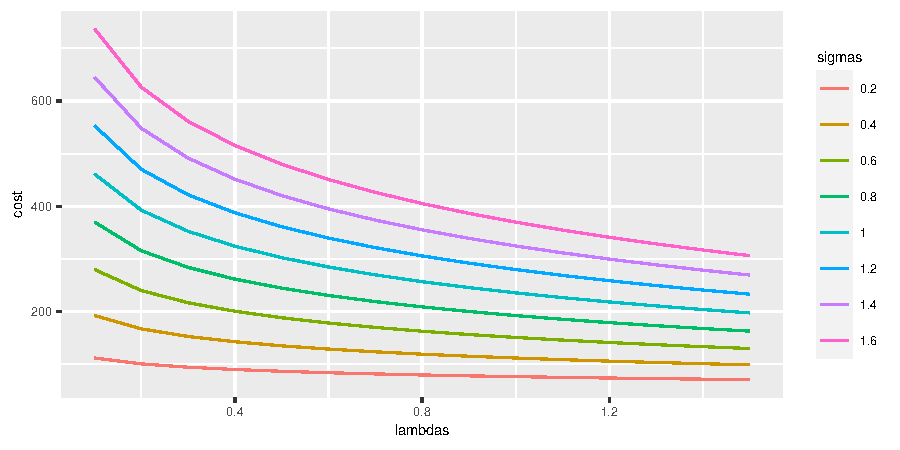
\includegraphics{figs/Chap4/only_cens.pdf}
    \caption{Plot of the cost function values against $\theta$ values when all observations are censored. It is represented for an exponential distribution. The sample consists in 100 values of censored observations to a threshold $a = 0.05$.}
    \label{fig:onlycens}
\end{figure}

We show in the next part why it could be problematic to have fully censored segments in the search method and how we chose to deal with it. 

\subsection{On the detection point method}

The case of fully censored segment are questionning the identifiability of the change-point detection method. The usual assumption \citep{Lavielle1997} for the segment parameters is the following:   
\begin{itemize}
\item[\textbf{H1:}] $\Theta$ is compact and there exists $\Delta_{\bm \theta}^{\star}>0$ such that $\vert \theta_{k+1}^{\star}-\theta_{k}^{\star}\vert > \Delta_{\bm \theta}^{\star}$, for all $k=0,...,K^{\star}$. 
\end{itemize}

We have seen in \ref{chp:4:costex} that, for the exponential distribution example, the optimal $\theta$ tends to infinity. If that is the case $\Theta$ is not compact. To solve this problem, we impose an upper bound $\theta_{max}$ on the possible values of $\theta$. Thus, we have that $\theta \in [0,\theta_{max}]$ which is a compact part of $\mathbbm{R}$. 

A new problem arises from this modeling choice. The value of $\theta_{max}$ must be chosen carefully. We must ensure that $\theta_{max}> \theta^*_k,$ for all $k \in \{0,\dots,K^*\}$. If it is not the case, the identification problem remains. For two $\theta^*_i$ and $\theta^*_j$    greater than $\theta_{max}$, their estimates will be set to $\theta_{max}$ and thus no segment identification will be possible. In order to avoid such problems, the value of $\theta_{max}$ is set according to the worst censoring case scenario possible. More precisely, we assume no change-point occured in $\bm y$ and that all observations are distributed according to $Q$ with parameter $\theta_{max}$. We set $\theta_{max}$ to the value such that: 
$$F(\min(\bm y),\theta_{max})^n = \alpha,$$
with $\alpha$ being a desired percentage of censorship. 

We provide a practical example with the exponential distribution. We simulate a signal $\bm y$ of size $n = 200$ that is a realization of exponential distributions of parameters $\theta^*_0 = 1$ for $y_{1:100}$ and $\theta^*_1 = 4$ for $y_{101:200}$. The censoring level is set to the median of $\bm y$ so that 50$\%$ of the signal is censored. We illustrates $\bm y$ in Figure \ref{fig:theta_max}. We set $\theta_{max}$ choosing with $\alpha = 95\%$. We have that $\theta_{max} = \frac{-\log(1-\alpha)}{\min(\bm y)}$. In our numerical example, $\theta_{max} = 10.56$, which is greater than $\theta_0$ and $\theta_1$.

\begin{figure}[ht]
    \centering
    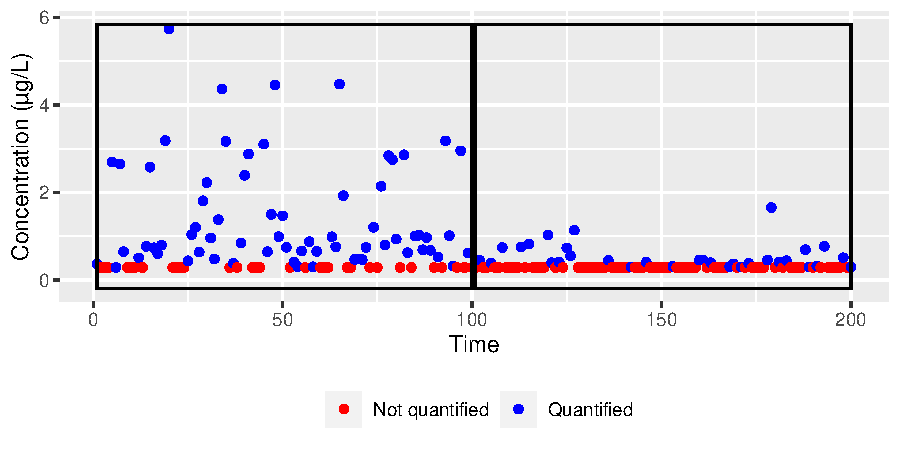
\includegraphics{figs/Chap4/theta_max_ex.pdf}
    \caption{Example of simulated signal $\bm y$ distributed according exponential distributions. The two segments are drawned with black rectangles. $\theta^*_0 = 1$ in the left segment, $\theta^*_1 = 4$ in the right one and the censoring threshold $a = 0.28$ in both segments}
    \label{fig:theta_max}
\end{figure}

\section{Estimation procedure}\label{chp:4:3}

We propose the following heuristic to estimate $\sigma$ and to calibrate the penalty term $\beta_n$. It consists in an iterative procedure where we alternate between optimizing \ref{mle:crit} with respect to $\sigma$ and $(L,\eta)$. The goal is to construct a sequence $\bm{\widehat{\sigma}} = (\widehat{\sigma})_{r=0}^R$ that converges to $\sigma^*$ when $R \to +\infty$ and then to retrieve the results of the best segmentation possible for the last $\widehat{\sigma}_r$ computed.
In the initialisation step, the estimate of $\sigma$ is computed from the whole signal $(\maxy_1,...,\maxy_K)$ by supposing that there is no change-point. More formally, it is equivalent to take the case where $L = 0$ and minimizing the cost: 
\begin{equation}\label{heu:init}
\mathcal{C}(\lambda,\sigma;   \overline{\mathcal{D}})= -\ln \mathcal L(\lambda,\sigma; \maxy_{1}, \ldots, \maxy_{K}) + \beta_K D,
\end{equation}
We proceed using the MLE estimator for both parameters $\lambda$ and $\sigma$, which implies using iterative methods again as stated in \cite{cohen1965maximum}, giving the estimators:
\begin{equation}\label{heu:sigma1}
(\widehat{\lambda}_0, \widehat{\sigma}_0) = \arg \min_{\lambda, \sigma} \mathcal{C}(\lambda, \sigma ;   \overline{\mathcal{D}}).
\end{equation}

It can be noted straight away that the value of $\widehat{\lambda}_0$ will be discarded since it was computed from a model that goes in direct contradiction with the assumptions we made in \ref{subsection:pwsm}. However, $\widehat{\sigma}_0$ is the starting point of our heuristic which can be described in two steps.
At the $r-$th iteration with $r \in [1:R]$:
\begin{enumerate}
    \item Minimise \ref{mle:crit} using the value of $\widehat{\sigma}_{r-1}$ to obtain:  
\begin{equation}\label{mle:crit2}
(\widehat{L}, \widehat{\bm{\eta}}) = \arg \min_{L, \bm{\eta}} \mathcal{C}(L,  \bm{\eta}, \widehat{\bm{\lambda}}_{MLE}(L, \bm{\eta}),\widehat{\sigma}_{r-1};   \overline{\mathcal{D}}).
\end{equation}
The change-points $\widehat{L}$ and the associated locations $\widehat{\bm{\eta}}$ are obtained by applying the PELT procedure \cite{Killick2012}, which improves the optimal partitioning approach through a lower, linear complexity. PELT is run several times on a penalty grid $(\beta_0,\dots,\beta_q,\dots,\beta_{Q})$ where $\beta_0<\dots<\beta_{q}<\dots<\beta_{Q}$. We obtain $Q$ (not necessarily unique) segmentations of $\overline{\mathcal{D}}$. Eventually, the optimal penalty value for this step is selected using an elbow rule heuristic as proposed in \cite{lung2015}: segmentation scores are plotted against their corresponding number of change-points $L$. One looks for the number of breaks $\hat L$ that minimizes the sums of squares of two linear models respectively fitted on the $L \geq \hat L$ and the $L \leq \hat L$. We define $(\widehat{L}_r,\widehat{\eta}_r,\widehat{\bm{\lambda}}^r_{MLE}(\widehat{L}_r,\widehat{\eta}_r))$ the estimators associated to the segmentation selected with the elbow heuristic. 
\item Compute $\widehat{\sigma}_r$. One can write the new negative log-likelihood of the whole signal $\overline{\mathcal{D}}$ defined by $(\widehat{L}_r,\widehat{\eta}_r,\widehat{\bm{\lambda}}^r_{MLE}(\widehat{L}_r,\widehat{\eta}_r))$ as a function of $\sigma$ as follows:
\begin{equation}\label{new:lk}
g(\sigma;   \overline{\mathcal{D}})=\sum_{l=1}^{\widehat{L}_r+1}  -\ln \mathcal L(\widehat{\lambda}_{r,l},\sigma; \maxy_{\widehat{\eta}_{r,l-1}+1}, \ldots, \maxy_{\widehat{\eta}_{r,l}}),
\end{equation}
where $\widehat{\lambda}_{r,l}$ is the $l-$th estimator in $\widehat{\bm{\lambda}}^r_{MLE}(\widehat{L}_r,\widehat{\eta}_r))$. $\widehat{\sigma}_r$ is found by minimizing \ref{new:lk} which can be perform using iterative procedures. 
\end{enumerate}

Simulation studies are available in Appendix \ref{app:sim:chap5} showing the convergence of this heuristic. Once a suitable value of $\sigma$ is obtained, the choice of the final penalty term $\beta_K$ is driven by the CROPS algorithm \cite{haynes2017}, which computes all optimal segmentations as the penalty varies over some interval. Eventually, the final penalty value is selected using an elbow rule heuristic.


\section{Simulation study}\label{chp:4:4}

\subsection{Experiments on the minimal segment length}

\textbf{The minimal segment length:} this argument is implicitly introduced when the number of changes $K^\star$ is not known. We want to calibrate this parameter by comparing the ability of our method to detect the presence of a change point in the data with the \textit{Multrank} method. In this context, comparing the non-parametric approach with the parametric approach is equivalent to using a likelihood ratio for the latter. It should be noted that performing a likelihood ratio test or maximising the penalised likelihood introduced in the Equation \ref{eq:ml-unknown-k} for $K_{max} = 1$ is equivalent whatever the choice of penalty might be. The statistics of the non-parametric test and the likelihood ratio test are calculated for each sample and will allow the calculation of the ROC curves \cite{Fawcett2006} and the corresponding areas under the curve (AUC) to compare the performances of the two approaches. The results obtained on the simulated data are shown in Figure \ref{fig:sim_minseg}. For both methods, the area under the ROC curve is calculated by varying the minimum number of observations before a change point. According to these results, the parametric method performs better when the interval between two interruptions contains enough observations. In addition, the performance of the two methods is also compared as a function of the censoring threshold. We choose to fix the minimum segment length value to 50 observations. We are assured that in a highly censored context the parametric method will perform correctly.   
    \begin{figure}[ht]
    \centering
    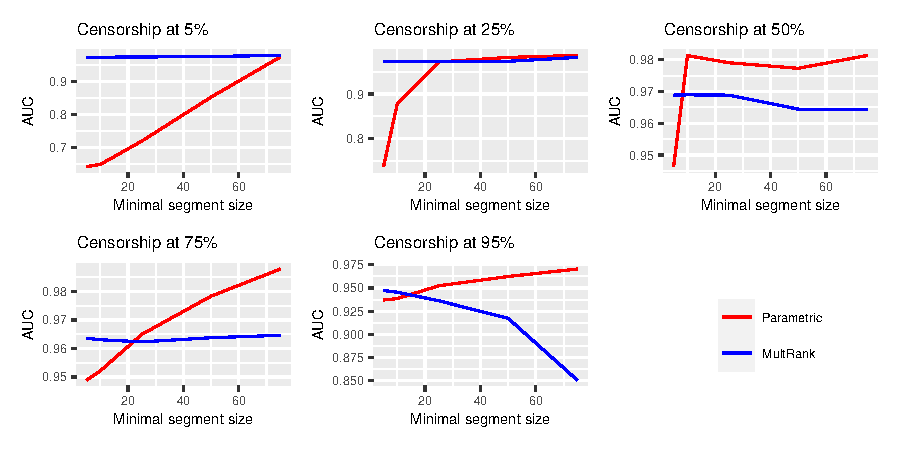
\includegraphics{figs/Chap4/sim_minseg.pdf}
    \caption{Choice of the minimal segment length: simulation results. Our method performance is Illustrated with the red line, the \textit{Multrank} method is drawn in blue. The results are illustrated for several censorship thresholds and the different minimal segment lengths used were $5,10,25,50$ and $75$ observations.}
    \label{fig:sim_minseg}
\end{figure}

\subsection{Comparison with a non parametric method}

\textbf{The penalty calibration:} The last parameter to be set is the penalty $\beta$. While calibrating $\beta$, we want to compare the performance of the break detection with the Multrank method. The experimental framework is as follows: 
    \begin{enumerate}
        \item we simulate $N=100$ samples $(x_1,...,x_n)$ of size $n=400$  following a left-censored Weibull distribution with $\alpha\%$ of censored data. We made tests for the different censorship rates $\alpha = (25,50,75,95)$. The shape parameter of the Weibull distribution is assumed to be known and set to $\sigma=0.5$. The scaling parameters $\bm{\lambda^\star}$ have $K^\star=4$ breaks at positions $p^\star_1 = 80$, $p^\star_2 = 160$, $p^\star_3 = 240$ and $p^\star_4 = 320$ and take the values $\bm{\lambda^\star}=(\lambda^\star_1 = 1, \lambda^\star_2 = 4, \lambda^\star_3 = 0.5, \lambda^\star_4 = 5, \lambda^\star_5 = 1)$. An example of a sample simulated in this way is shown in Figure \ref{fig:ex_sim}.
        \item For each of the $N$ samples, we perform the parametric change-point detection and the Multrank methods. For each sample, we obtain the estimated number of breaks $\hat K_{param}$ and $\hat K_{multrank}$ and their position $(\hat{p}_{k,param})_{k = 1}^{\hat K_{param}}$ (respectively $(\hat{p}_{k,multrank})_{k = 1}^{\hat K_{multrank}}$).
        \item for both methods, we count the number of samples among the $N$ for which the correct number of breaks has been estimated (e.g. $\hat K_{param} = K^\star$). Also, for each of the samples for which the estimate of $K^\star$ is correct, we examine the distance between the estimated position of a change-point and its nearest true break $\min_{k,i \in [1:K^*]}(\hat{p}_{k} - p^\star_i)$. 
    \end{enumerate}
    In the case where $K$ is not known, we proceed as follows for each method to estimate it:
    \begin{itemize}
        \item For the parametric method: we use the algorithm CROPS, algorithm to scan a continuous range of penalty values $[\beta_{min},\beta_{max}]$. We obtain a set of $B$ values $(\hat \beta_1,...,\beta_B)$ and the optimal segmentations associated with these penalty values. We then plot the cost of the segmentations as a function of the number of breaks. We choose the optimal penalty using a elbow heuristic. This procedure is described in \cite{haynes2014}. The choice of $\beta_{min}$ and $\beta_{max}$ is inspired from linear penalties like the BIC criterion \cite{YAO1988181}. Note that when using the BIC penalty in change point detection, the penalty term written in section \ref{sub:pelt} becomes : $\beta_n = \frac{D}{2}\log(n) = \frac{1}{2}\log(n)$, where $D$ is the number of dimensions of the parameter. More precisely, we took a wide interval of penalty values defined by $\beta_{min} = \frac{\log(n)}{10}$ and $\beta_{max} = 5\log(n)$.
        \item For the non parametric \textit{Multrank} method, we compute the optimal segmentation for $k$ breaks, where $k$ ranges from $1$ to $K_{max}$. For each of these segmentations, we can compute the value of the statistic $I_k(n)$ statistic described in \cite{lung2015}. As in the parametric method, we represent the values of this statistic as a function of $k$, and we determine the number of estimated breaks by an elbow heuristic. Here, $K_{max}$ is fixed at $2*K^\star = 8$.
    \end{itemize}
The results of the simulations are shown in Table \ref{tab:simcomp} and in Figure \ref{fig:prec_sim}. It can be seen that in the ideal scenario, where the data are indeed distributed according to a left-censored Weibull distribution, the parametric method performs better both in detecting the correct number of breaks and in accurately estimating their position. However, this performance decreases as the censoring rate increases.

\begin{figure}[ht]
    \centering
    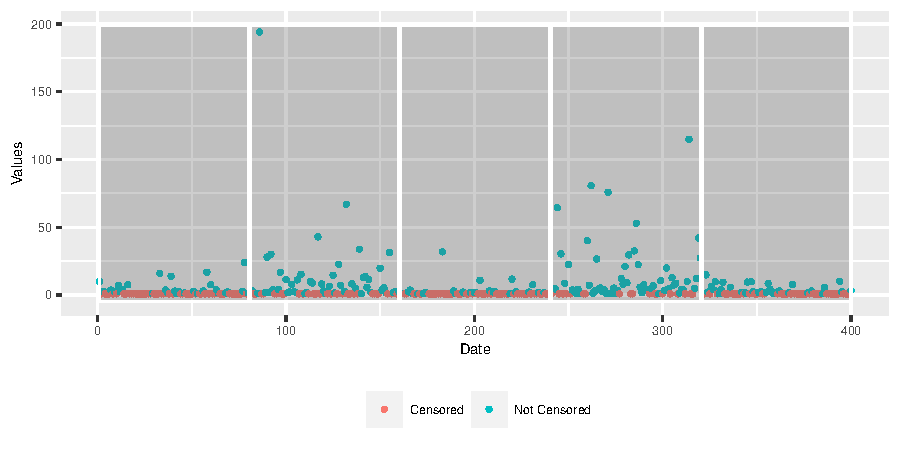
\includegraphics{figs/Chap4/Ex_sim.pdf}
    \caption{Example of simulated signal with $(\lambda_1 = 1, \lambda_2 = 4, \lambda_3 = 0.5, \lambda_4 = 5, \lambda_5 = 1)$, $\sigma = 0.5 $, $n = 400$, $K = 4$, $(p_1 = 80,p_2 = 160,p_3 = 240,p_4 = 320)$ and $\alpha = 50\%$.}
    \label{fig:ex_sim}
\end{figure}

\begin{table}[ht]
\centering
\begin{tabular}{|r|r|r|}
  \hline
   $\alpha(\%)$  & Parametric method & MultRank \\ 
  \hline
 25 &  84 &  58 \\ 
 50 &  80 &  63 \\ 
 75 &  87 &  68 \\ 
 95 &  65 &  10 \\ 
   \hline
\end{tabular}
\caption{Number of correct estimations of $K$ over $N=100$ samples for both methods for different $\alpha\%$ censorship rates.}
\label{tab:simcomp}
\end{table}

\begin{figure}[ht]
    \centering
    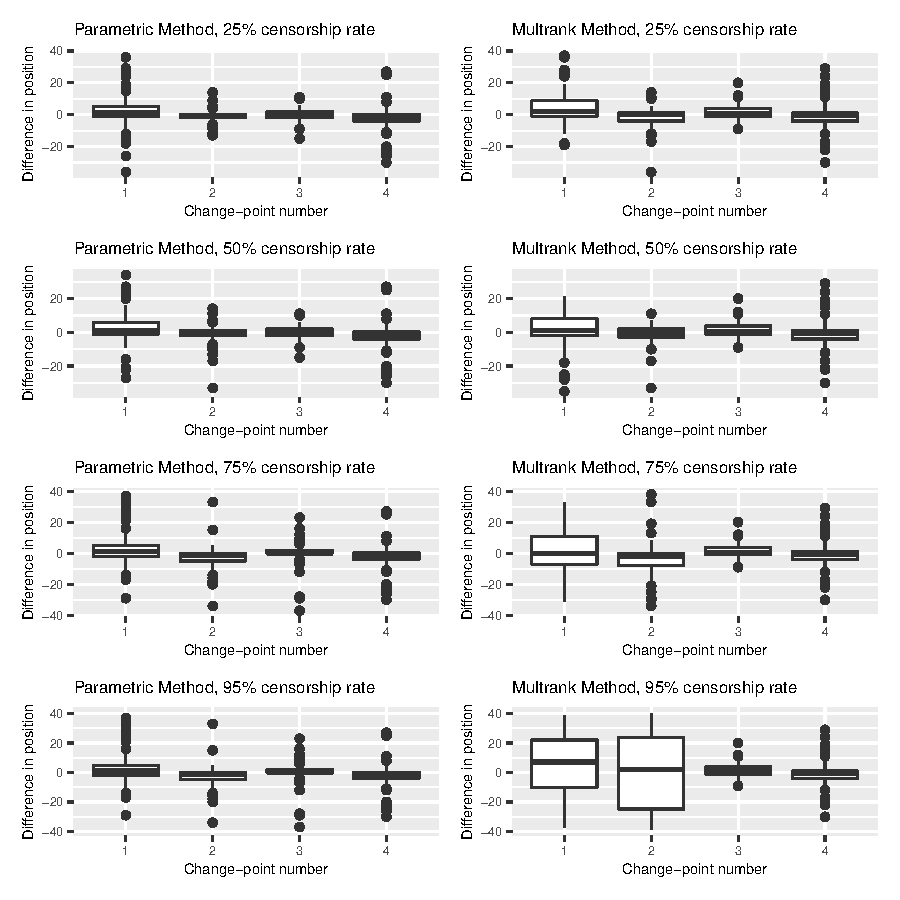
\includegraphics{figs/Chap4/P_RUPT.pdf}
    \caption{Precision of the estimated change-points for both methods.}
    \label{fig:prec_sim}
\end{figure}
